\documentclass[lmodern, utf8, seminar]{fer}
\usepackage{booktabs}
\usepackage{graphicx}
\usepackage{float}

\graphicspath{ {images/} }

\begin{document}
\nocite{*}



\title{Suparnički generativni modeli za prevođenje slika}

\author{Krešimir Vukić}
\voditelj{prof.~dr.~sc.~Siniša Šegvić}

\maketitle


\tableofcontents



\chapter{Uvod}
Generiranje slika na temelju skice, prijenos stilova i rekonstrukcija fotografije samo su neki od problema računalnog vida. Pri njihovom rješavanju uglavnom želimo naučiti funkciju mapiranja između parova slika koju zatim koristimo za efikasnu identifikaciju značajki ili po potrebi, njihovo generiranje. 

Među najkorištenijim i najuspješnijim arhitekturama današnjice nalaze se generativni suparnički modeli. Ovim radom istražiti će se različita proširenja kojima se ti modeli prilagođavaju specifičnim problemima, njihove karakteristike i primjene.

\chapter{Duboke mreže}
Duboke neuronske mreže zadnjih godina izuzetno su popularne u rješavanju klasifikacijskih problema i pronalaženju uzoraka. Tome je zaslužna prednost koju imaju naspram klasičnih pristupa, a koja se očituje u vidu mogućnosti da samostalno pronalaze bitne značajke u podatcima te na temelju njih i tražena rješenja.

Slojevit pristupu rastavljanja podataka na jednostavnije građevne jedinice čini ih posebice prigodnima za radu sa problemima hijerarhijske prirode poput slika. 
\newline

\section{Konvolucija}
Konvolucijske mreže osmišljene su s ciljem dohvata lokalnih relacija među podatcima koje se posebice očituju pri radu sa slikama. Naime, ukoliko želimo analizirati malenu značajku na slici, nepoželjno je da njena pozadina ili lokacija unutar slike utječe na nju samu. 

Ideja konvolucije je da se kao ulaz u neurone sljedećeg sloja dovede više vrijednosti s prethodnog što je prikazano slikom \ref{fig:convolution}. To se odvija tako da se unaprijed definiran kvadrat pomiče (konvoluira) po ulaznim podatcima i tako određuje mapiranje na sljedeći sloj. Rezultat tog procesa je da pridodajemo veću važnost pikselima u neposrednoj okolini istraživanog područja.
\newline

\begin{figure}[H]
    \centering
    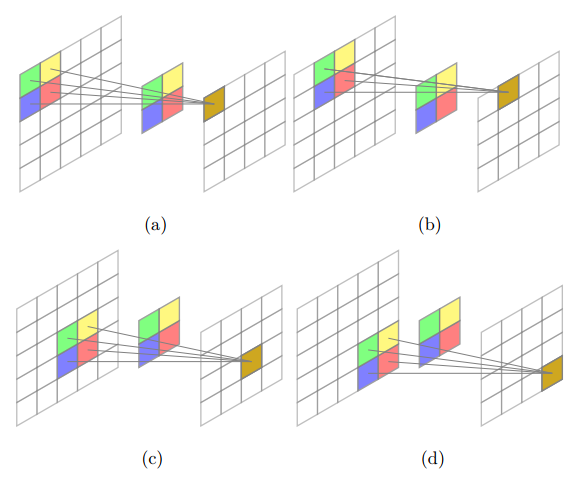
\includegraphics[width=0.8\textwidth]{convolution}
    \caption{Proces konvolucije}
    \label{fig:convolution}
\end{figure}

\section{Primjer konvolucijske mreže}
Nizanjem konvolucijskih slojeva dobivamo arhitekturu u kojoj je svaki sloj zadužen za jednostavniji potproblem sljedećeg sloja. Na slici \ref{fig:dnn} prikazana je duboka neuronska mreža s 5 konvolucijskih slojeva među kojima se odvija sažimanje maksimalnom vrijednošću te dva sloja potpune povezanosti.
\newline

\begin{figure}[H]
    \centering
    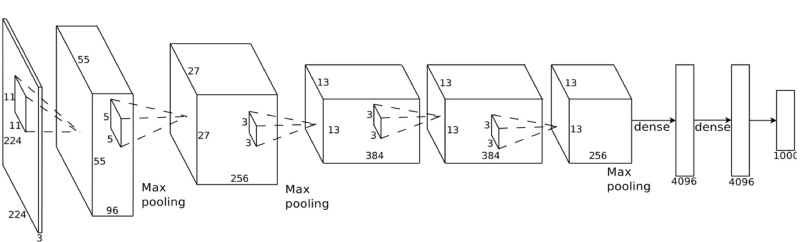
\includegraphics[width=0.9\textwidth]{dnn}
    \caption{Primjer duboke neuronske mreže}
    \label{fig:dnn}
\end{figure}

\chapter{Generativni suparnički modeli (GAN-ovi)}
GAN-ovi su podvrsta dubokih mreža čija arhitektura se bazira na dvije podmreže koje uče kroz međusobno natjecanje. Tako nespecifični model, ovisno o implementaciji, u stanju je kopirati distribuciju širokog spektra podataka: slika, govora, muzike, čak i pisanih zapisa.
\newline

\section{Generativni naspram diskriminativnih algoritama}
Dvije temeljne skupine koijima dijelimo algoritme za učenje su diskriminativni i generativni.
Njihovi nazivi dolaze izravno iz vrste problema koji riješavaju: 
\newline

Diskriminativni modeli direktno mapiraju ulazne varijable na ciljne vrijednosti i time uče uvjetnu vjerojatnost $p(Y|X)$. Dobiveni model svrstava podatke u ciljne klase s određenom vjerojatnošću.

Generativni modeli, kao što im i naziv govori, generativne su prirode. Problem koji riješavaju je kako dobiti $X$ uz dani $Y$, tj. pokušavaju naučiti distribuciju pojedinih klasa $p(X \mid Y)$.
\newline

Drugim riječima, dok diskriminativni modeli pokušavaju pronaći granicu između klasa, generativni modeliraju distribucije pojedinih klasa na temelju kojih mogu uzorkovati nove primjere.
\newline

\section{Rad GAN-a}
Pola mreže bavi se stvaranjem novih podataka dok druga polovica pokušava evaluirati koliko su slični stvarnim podatcima.
Cijeli proces usporedljiv je s poslovima detektiav i kriminalca. Jedna strana u bavi se falsifikacijom dokaza, a druga analizom njihove autentičnosti.
\newline

Koraci rada GANa:
\begin{enumerate} 
\item generator iz nasumičnih brojeva stvara sliku
\item ta slika se dovodi na ulaz diskriminatora uz skup stvarnih slika iz podatkovnog skupa
\item diskriminator određuje postotak vjerojatnosti da je slika prava
\end{enumerate}



\chapter{Uvjetne generativne mreže}
Uvjetne generativne mreže pokazale su se kao generalno rješenje problema prevođenja slike [pix2pix]. Svojstvene su po učenju ne samo funkcije prijenosa između slika već i funkcije gubitka nad kojom se ona trenira.
Dok se u drugim modelima ona ručno zadaje, pristup u kojem se ona uči omogučuje generalizaciju nad setovima problema koji bi u suprotnom zahtijevali vrlo drugačije formulacije gubitka.
\newline

\section{Primjena}
Neke od mogućnosti uvjetnih GAN-ova su sinteza fotorealističnih slika iz skica, generiranje objekata na temelju njihovih obruba te bojanje crno bijelih fotografija.



\chapter{Translacija bez uparenih primjera za učenje pomoću kružnih GAN-ova}
\section{Prednosti}
Većina postojećih algoritama korištenih u računalnom vidu ovisi o postojanju velikih podatkovnih setova označenih parova slika. No, za mnoge probleme takvi podatci nisu dostupni, a u takvim situacijama primjenu nalaze kružni GANovi.
\newline

\section{Rad CycleGAN-a}
Temelj njihovog rada je uz da uz učenje funkcije $G: X \rightarrow Y$, istovremeno uče njen inverz $F: X \rightarrow Y$ pomoću gubitka cikličke dosljednosti: $F(G(X)) \approx X$ i obrnuto.
\section{Primjena}


\chapter{Prijenos stila}




\chapter{Zaključak}




\bibliography{literatura}
\bibliographystyle{fer}



\begin{sazetak}
Mnogi problemi u procesiranju slika odnose se na translaciju ulazne slike u željenu izlaznu. Većina današnjih arhitektura bazira se na generativnim suparničkim mrežama, nad kojima su osmišljena mnoga proširenja kako bi se prilagodila specifičnim problemima. Uvjetnim generativnim mrežama nije potrebno definirati funkciju gubitka jer ju mogu same naučiti, kružne generativne mreže sposobne su učenju translacije ne samo ulaznih u izlazne primjere nego i u drugom smjeru, a ograničavanjem mreže na translaciju unutar prostora boja obavljat će prijenos stila bez distorzije sadržaja slike. Ovim radom usporedit ću različite arhitekture, njihove karakteristike i primjene na problemima translacije slike u sliku.

\kljucnerijeci{image-to-image generation, style transfer, GANs, CycleGANs}
\end{sazetak}

\engtitle{Image to image generation using CycleGANs}
\begin{abstract}

\keywords{image-to-image generation, style transfer, GANs, CycleGANs}
\end{abstract}

\end{document}